% SN 2024pba — Two-Event Interacting-Supernova Scenario
% Companion document to scenario.md; figures produced by
% scripts/make_scenario_figures.py
%
% Compile: module load texlive/2021
%          pdflatex scenario && bibtex scenario && pdflatex scenario && pdflatex scenario

\documentclass[11pt, a4paper]{article}

\usepackage[round, sort, compress]{natbib}
\usepackage{amsmath, amssymb}
\usepackage{graphicx}
\usepackage{booktabs}
\usepackage{hyperref}
\usepackage[T1]{fontenc}
\usepackage{microtype}

\newcommand{\Msun}{\ensuremath{M_\odot}}
\newcommand{\kms}{\ensuremath{\mathrm{km\,s^{-1}}}}
\newcommand{\Ni}{\ensuremath{^{56}\mathrm{Ni}}}
\newcommand{\SNa}{SN$_{\mathrm{A}}$}
\newcommand{\SNb}{SN$_{\mathrm{B}}$}

\begin{document}

\title{SN~2024pba as a Two-Event Interacting Supernova:\\
       Model Scenario and Current Evidence}
\author{S. Brennan\\
\small Max Planck Institute for Astrophysics, Garching, Germany}
\date{\today}

\maketitle

\begin{abstract}
\noindent
SN~2024pba is modelled as \emph{two interacting explosion events} rather than
a single supernova: an earlier Type~IIb explosion (\SNa) that left fast,
metal-rich ejecta, and a later event (\SNb) whose dense shell is launched
into the space inside the aged \SNa\ ejecta and drives an embedded shock.
This note summarises the observational anchors, the model parameterisation,
and the mechanism that produces a double-peaked lightcurve, and identifies
the outstanding test: whether radiative heating of the metal-rich \SNa\
ejecta reproduces the observed absorption spectrum.  All figures are
reproducible from the pipeline data via
\texttt{scripts/make\_scenario\_figures.py}.
\end{abstract}

\section{Observational anchors}
\label{sec:obs}

Figure~\ref{fig:obs_lc} shows the ATLAS lightcurve of SN~2024pba in absolute
magnitude ($o$ and $c$ bands).  The two events are separated by
$\sim$330--360~d: the first, fainter maximum (\SNa) peaks near MJD~60513 at
$M\approx-17.2$, and the main event (\SNb) peaks at MJD~60850 with
$o\approx-18.2$, preceded by a $\sim$30--40~d precursor bump near
MJD~60810--60830.  Table~\ref{tab:anchors} lists the adopted anchors and
distance/extinction.  The interval between the events implies that any
material connecting them has had $\sim$1~yr of homologous expansion, which
sets the radial scale of the interaction region ($\sim$10$^{16}$~cm for
typical ejecta velocities of a few $10^3$~\kms).

\begin{figure}[t]
  \centering
  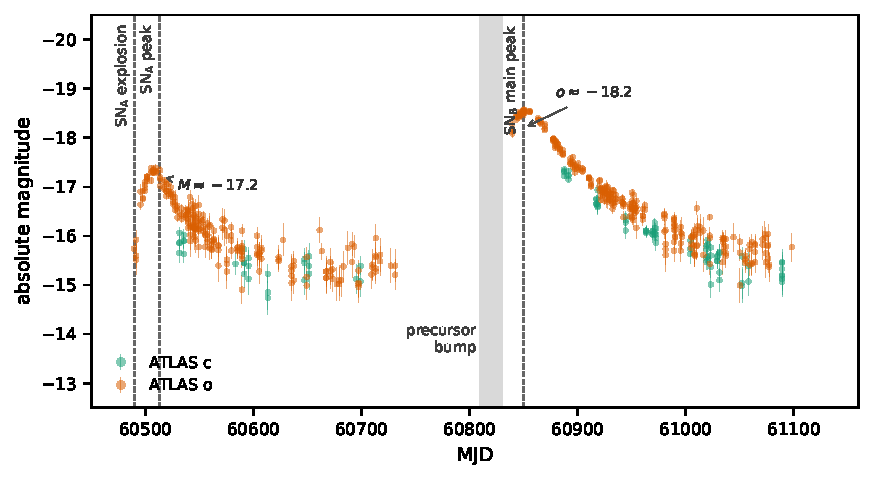
\includegraphics[width=\columnwidth]{figures/fig_obs_lc.pdf}
  \caption{ATLAS $o$- (orange) and $c$-band (cyan) lightcurve of SN~2024pba in
  absolute magnitude ($D_L=80.4$~Mpc, $E(B{-}V)=0.15$).  Dashed lines mark the
  adopted anchors: \SNa\ explosion ($\sim$MJD~60490, constrained by the ATLAS
  rise), \SNa\ peak (60513), and the \SNb\ main peak (60850).  The grey band
  marks the precursor-bump window, $\sim$30--40~d before the main peak.
  A few bad-subtraction outliers have been removed.}
  \label{fig:obs_lc}
\end{figure}

\begin{table}[t]
  \centering
  \caption{Observational anchors and adopted distance/reduction.}
  \label{tab:anchors}
  \begin{tabular}{lll}
    \toprule
    Quantity & Value & Note \\
    \midrule
    \SNa\ explosion & $\sim$MJD 60490 & ATLAS rise of first event \\
    \SNa\ peak & MJD 60513, $M\approx-17.2$ & fainter first maximum \\
    \SNb\ precursor bump & $\sim$MJD 60810--60830, $M\approx-15.8$ &
      shock-cooling bump \\
    \SNb\ main peak & MJD 60850, $o\approx-18.2$ & lightcurve reference \\
    $D_L$ & 80.4~Mpc (DM $=34.53$) & $z=0.0186$ \\
    $E(B{-}V)$ & 0.15 & $A_o\approx2.40\,E$ \\
    \midrule
    \SNa\ expl.\ $\rightarrow$ \SNb\ peak & $\approx360$~d & \\
    Interaction onset & $\sim$320--340~d after \SNa & bump 30--40~d pre-peak \\
    \bottomrule
  \end{tabular}
\end{table}

Figure~\ref{fig:spectra} shows the two available optical spectra.  The DBSP
spectrum (MJD~60523.5, $\sim$10~d after the \SNa\ peak) belongs to the first
event; the ALFOSC spectrum (MJD~60875.1, $+25$~d after the \SNb\ peak) samples
the main event.  The scientific requirement on the scenario is that the strong
H, He, O, Si, Ca and Fe absorption seen in these spectra be physically
attributed --- ion, transition, formation radius and velocity --- and in
particular be testable against the hypothesis that the lines form in the
radiatively heated \SNa\ ejecta rather than in the \SNb\ shell/CSM alone.

\begin{figure}[t]
  \centering
  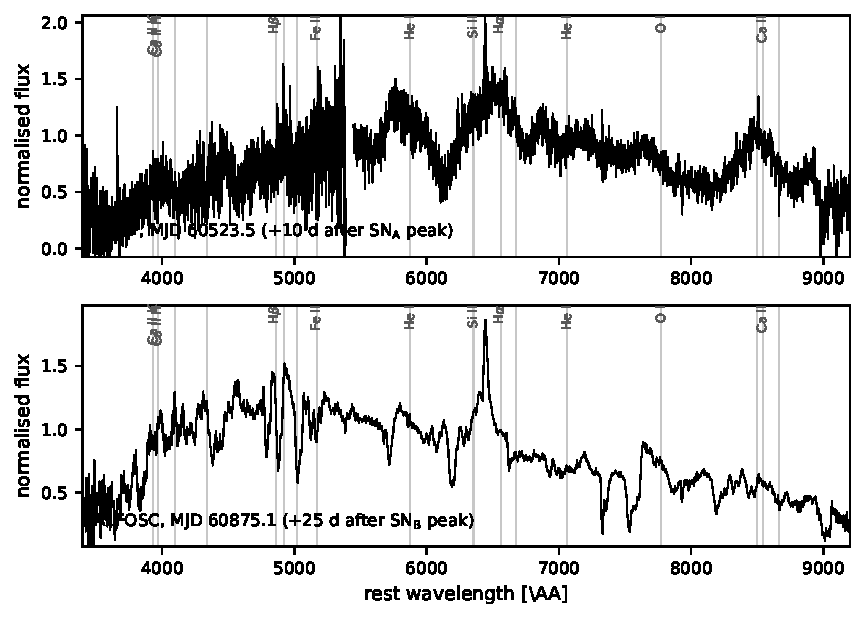
\includegraphics[width=\columnwidth]{figures/fig_spectra.pdf}
  \caption{Observed spectra of SN~2024pba, rest-frame ($z=0.0186$),
  normalised to the 5000--7000~\AA\ median.  Top: Palomar DBSP spectrum at
  MJD~60523.5, ten days after the \SNa\ peak.  Bottom: NOT ALFOSC spectrum at
  MJD~60875.1, 25~d after the \SNb\ main peak.  Grey lines mark the rest
  wavelengths of the key H, He, O, Si, Ca and Fe features.}
  \label{fig:spectra}
\end{figure}

\section{The two events}
\label{sec:events}

Figure~\ref{fig:schematic} illustrates the adopted geometry at the time of the
second event.

\begin{figure}[t]
  \centering
  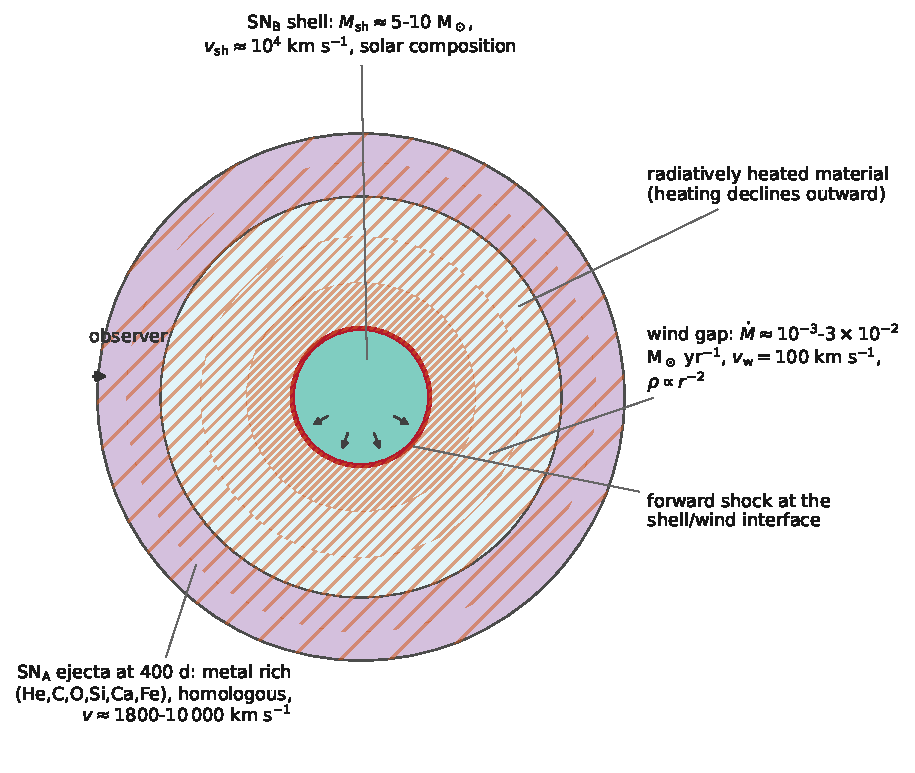
\includegraphics[height=0.5\textheight]{figures/fig_schematic.pdf}
  \caption{Schematic of the two-event geometry at \SNb\ shell launch
  (\SNa\ age $\approx400$~d; the wind$\rightarrow$ejecta buffer is omitted
  for clarity).  From inside out: the \SNb\ shell (solar composition,
  $M_{\rm sh}\approx5$--$10~\Msun$, $v_{\rm sh}\approx10^4$~\kms); the wind
  gap ($\rho\propto r^{-2}$); and the metal-rich, homologously expanding
  \SNa\ ejecta.  The forward shock (red) sits at the shell/wind interface;
  the orange hatching marks the radiatively heated material ahead of it,
  with the heating declining with distance from the interface.  The \SNa\
  ejecta is heated radiatively, not shocked.}
  \label{fig:schematic}
\end{figure}

\subsection{\SNa\ --- the first (Type~IIb) explosion}
\label{sec:sna}

\SNa\ is represented by the model \texttt{SN\_A\_g\_T20k\_Ni06}: a stripped
KEPLER progenitor (\texttt{s12.0-presn-stripped}, mass cut $1.4~\Msun$) with a
thin extended hydrogen envelope ($0.05~\Msun$, $R=200~R_\odot$,
$T_{\rm base}=20$~kK), explosion energy $\sim$9~B and $0.06~\Msun$ of \Ni.
The explosion produces fast, metal-rich (He/C/O/Si/Ca/Fe) ejecta that expand
homologously for $\sim$1~yr before the second event.
Figure~\ref{fig:sn_a_lc} compares the STELLA \citep{Blinnikov1998,
Blinnikov2006} lightcurve of this model with the observed first peak: the
model reproduces the observed $\sim-17$~mag maximum scale.

\begin{figure}[t]
  \centering
  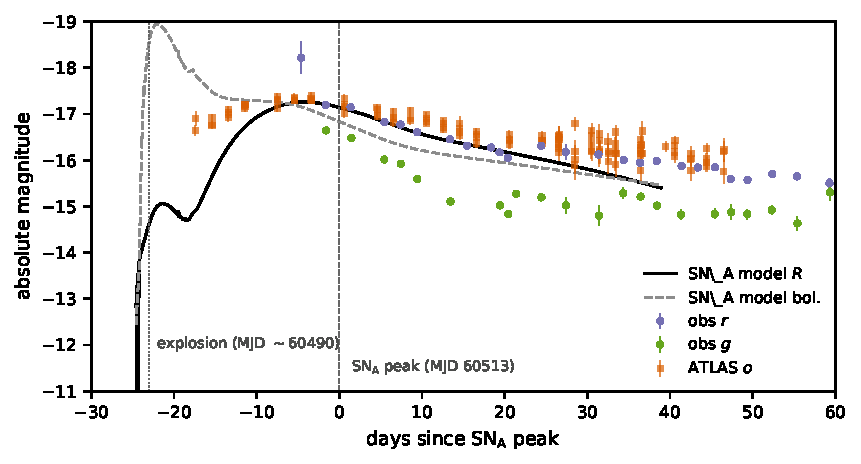
\includegraphics[width=\columnwidth]{figures/fig_sn_a_lc.pdf}
  \caption{\SNa\ model \texttt{SN\_A\_g\_T20k\_Ni06} $R$-band (solid) and
  bolometric (dashed) lightcurve, with the explosion epoch aligned to
  MJD~60490, compared to the observed $r$, $g$ and ATLAS $o$ photometry around
  the first peak.  The model reaches $M_R\approx-17.3$, close to the observed
  $-17.2$; the early bright phase is shock breakout through the extended
  envelope.}
  \label{fig:sn_a_lc}
\end{figure}

\subsection{\SNb\ --- the second event}
\label{sec:snb}

\SNb\ is represented not as a fresh full ejecta but as a \emph{dense shell}
($M_{\rm shell}\approx5$--$10~\Msun$, $v_{\rm shell}\approx10^4$~\kms, solar
composition) launched into the environment of the aging \SNa\ ejecta.  The
region between the shell and the \SNa\ ejecta inner edge is filled with a
steady wind ($\dot M_{\rm wind}\approx10^{-3}$--$3\times10^{-2}~\Msun\,
\mathrm{yr}^{-1}$, $v_{\rm wind}=100$~\kms, $\rho\propto r^{-2}$) plus a
smoothed wind$\rightarrow$ejecta buffer controlled by
\texttt{we\_transition\_dex}.

Figure~\ref{fig:input} shows the actual initial structure fed to STELLA for
the completed model \texttt{T6k\_M10.0\_V10000}.  The four regions ---
solar-composition shell, $\rho\propto r^{-2}$ wind gap, the
wind$\rightarrow$ejecta buffer, and the metal-rich \SNa\ ejecta --- are
clearly separated in both density and composition.  The velocity field is
deliberately non-monotonic: the shell peaks at $10^4$~\kms, the wind gap is
nearly stationary, and the \SNa\ ejecta resumes homologous expansion
($v\propto r$) reaching $10^4$~\kms\ at the outer edge.

\begin{figure}[t]
  \centering
  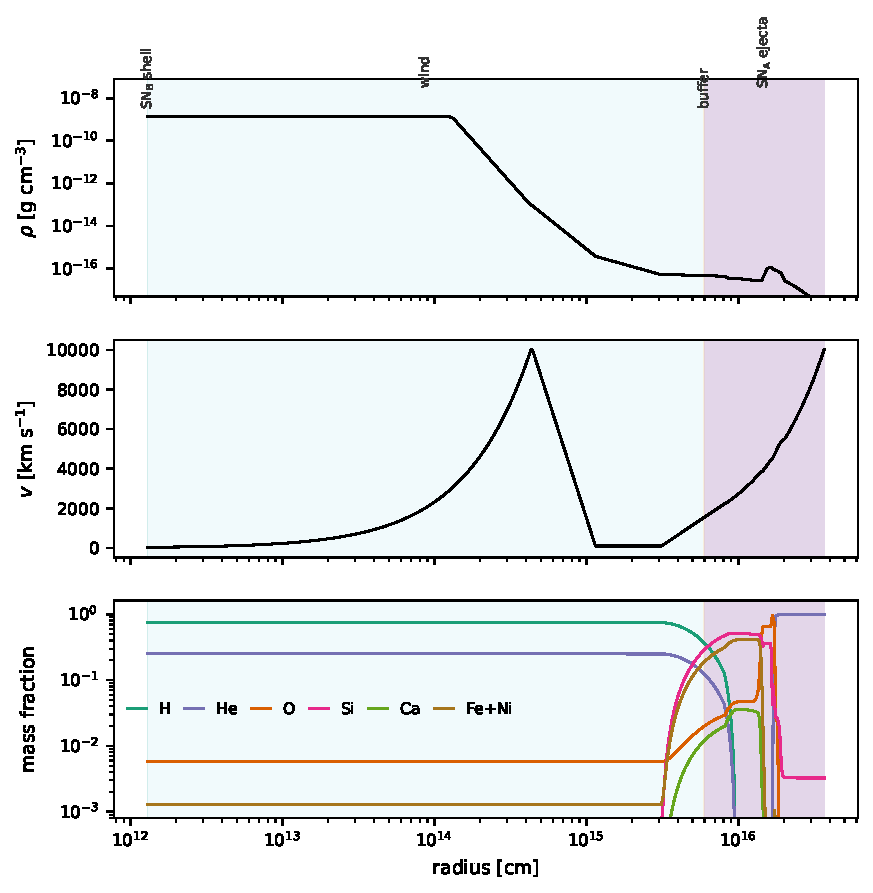
\includegraphics[width=0.85\columnwidth]{figures/fig_input_structure.pdf}
  \caption{Initial STELLA input structure of \texttt{T6k\_M10.0\_V10000}:
  density (top), velocity (middle) and mass fractions (bottom) versus radius.
  Shading marks the \SNb\ shell (teal), the wind gap (blue), the
  wind$\rightarrow$ejecta buffer (orange) and the metal-rich \SNa\ ejecta
  (purple).  The ejecta carries the He/C/O/Si/Ca/Fe reservoir whose
  radiative heating is the key spectral hypothesis.}
  \label{fig:input}
\end{figure}

\section{What makes the lightcurve double-peaked}
\label{sec:twopeaks}

Figure~\ref{fig:model_lc} shows the STELLA lightcurve of
\texttt{T6k\_M10.0\_V10000} against the observations, phased to each curve's
own maximum.  Two components are visible in both model and data:

\begin{enumerate}
  \item \textbf{First bump} ($M\approx-16.3$, $t\approx10$--40~d after
    launch): shock-cooling/diffusion.  The shell launched at $\sim10^4$~\kms\
    immediately shocks the optically thick wind; the deposited energy diffuses
    out on the $\sim$30~d wind diffusion time.  Its duration is set by the
    shock crossing time of the wind gap ($\sim4\times10^{14}\rightarrow
    \sim8\times10^{15}$~cm at 3000--5000~\kms).  This corresponds to the
    observed precursor bump ($\sim-15.8$, grey band).
  \item \textbf{Main peak} ($M\approx-19.4$ at $t\approx55$--60~d,
    $T_{\rm bb}\approx10^4$~K): the embedded shock rams into the dense
    wind--ejecta buffer, where the density rises by $\sim$1~dex across the
    transition, boosting the dissipation ($\propto\rho v^3$) while the
    remaining wind column ahead of the shock goes optically thin and releases
    the stored radiation.
\end{enumerate}

\begin{figure}[t]
  \centering
  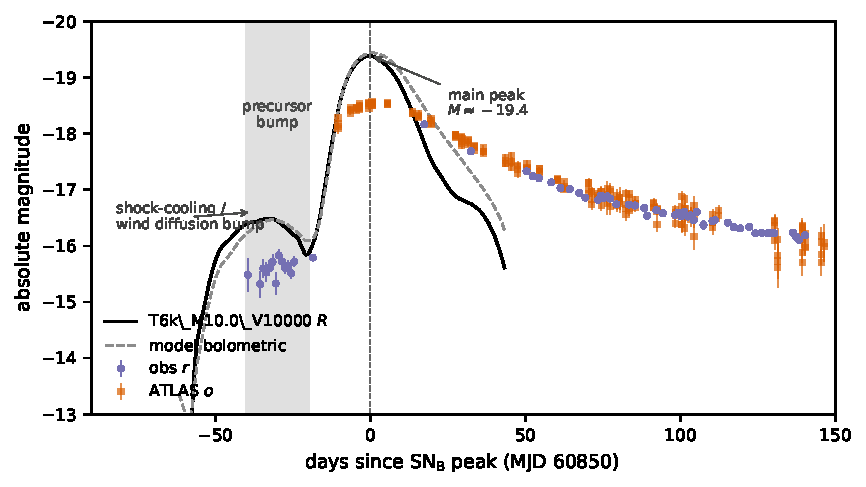
\includegraphics[width=\columnwidth]{figures/fig_model_lc.pdf}
  \caption{\texttt{T6k\_M10.0\_V10000} $R$-band (solid) and bolometric
  (dashed) lightcurve versus the observed $r$ and ATLAS $o$ photometry, phased
  to each curve's own maximum (model bands are Johnson--Cousins; systematic
  offsets of 0.1--0.3~mag vs.\ SDSS/ATLAS are expected).  The model reproduces
  the two-component morphology: a $\sim-16.3$~mag cooling/diffusion bump
  followed by a $\sim-19.4$~mag interaction-powered main peak.}
  \label{fig:model_lc}
\end{figure}

\subsection{Radiative heating, not shock heating, at maximum}
\label{sec:heating}

The distinguishing feature of the scenario is that \emph{at main peak the
\SNa\ ejecta is radiatively heated, not shocked}.  Figure~\ref{fig:heating}
shows the radial structure of \texttt{T6k\_M10.0\_V10000} at $t=20$, 40, 57
and 75~d from the completed STELLA run:

\begin{itemize}
  \item The forward shock --- visible as the velocity discontinuity (dotted
    lines) --- sits at $r\approx3$--$7\times10^{15}$~cm, roughly
    $10^{16}$~cm \emph{inside} the metal-rich ejecta inner edge (dashed lines,
    $X_{\rm O}>0.05$) throughout this interval; in this model true
    shock--ejecta contact has not occurred by $t\approx85$~d.
  \item The gas temperature at the ejecta face (dots, bottom panel) rises
    from $\sim2800$~K at $t=20$~d to $\sim6900$~K at $t=40$~d and remains
    $\sim5400$~K at maximum ($t=57$~d), well above the $\sim2200$~K adiabatic
    floor of the unshocked material --- the signature of the radiative
    precursor.  Note $T_{\rm gas}>T_{\rm rad}$ throughout the gap and ejecta:
    the heating is deposited in the gas, and a nebular/dilute-LTE ionisation
    estimate would be inappropriate.
  \item The ejecta velocity field stays homologous ($v\propto r$ across the
    whole O-rich region); no propagating velocity discontinuity reaches the
    metal-rich gas during the photospheric phase.
\end{itemize}

The metal-rich ejecta therefore acts as a \emph{radiatively heated screen} at
unperturbed \SNa\ velocities ($\sim1800$--$10\,000$~\kms) --- the proposed
source of the observed H, He, O, Si, Ca and Fe absorption.  Whether the
heating is sufficient to produce the observed line strengths at the observed
velocities is the pending CMFGEN test (Section~\ref{sec:open}).

\begin{figure}[t]
  \centering
  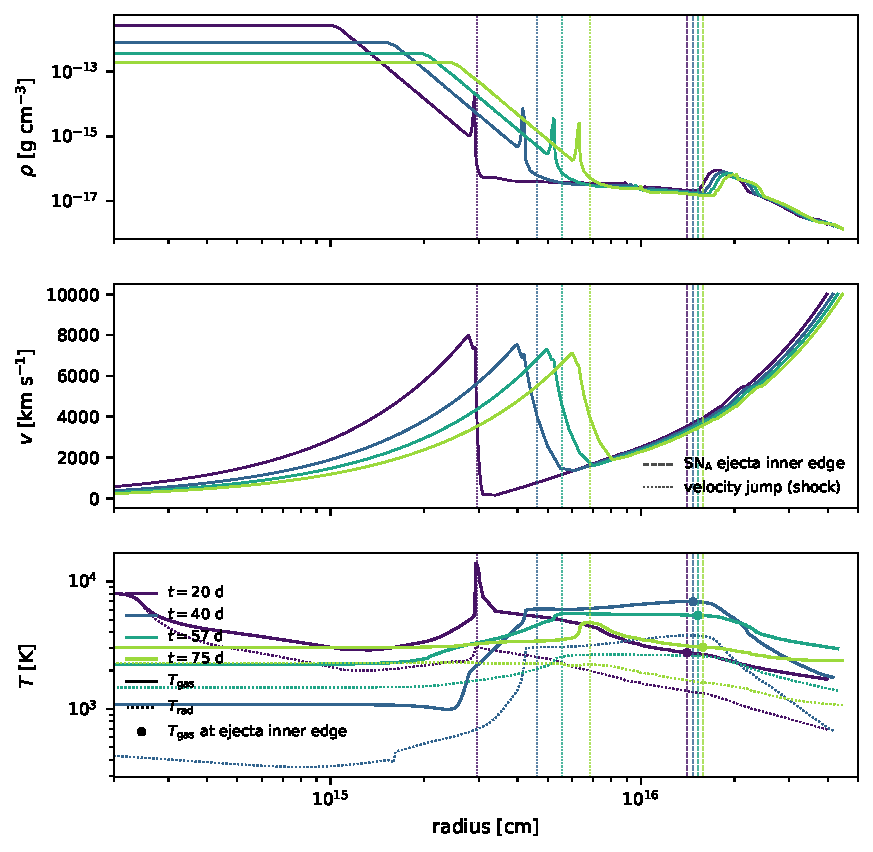
\includegraphics[width=0.85\columnwidth]{figures/fig_heating.pdf}
  \caption{Radial structure of \texttt{T6k\_M10.0\_V10000} from the STELLA
  \texttt{.swd} at $t=20$, 40, 57 and 75~d after shell launch (colour-coded).
  Top: density.  Middle: velocity.  Bottom: gas temperature (solid) and
  radiation temperature (dotted).  Dashed vertical lines mark the inner edge
  of the O-rich \SNa\ ejecta ($X_{\rm O}>0.05$); dotted lines mark the largest
  velocity discontinuity inside it (the embedded shock).  The ejecta face is
  heated radiatively while its velocity field remains homologous.}
  \label{fig:heating}
\end{figure}

\section{Model parameterisation: the \texttt{X\_*} grid}
\label{sec:grid}

All production models are generated and submitted through
\texttt{scripts/run\_model\_grid.py}, with the naming convention
\texttt{X\_M\{mass\}\_V\{velocity\}[\_W\{mdot\}][\_we\{dex\}]}.
Table~\ref{tab:grid} lists the explored parameters; the \SNa\ ejecta age at
shell launch is fixed at 400~d by the observed event separation.

\begin{table}[t]
  \centering
  \caption{Grid parameters and their established lightcurve roles.}
  \label{tab:grid}
  \begin{tabular}{lll}
    \toprule
    Parameter & Values & Controls \\
    \midrule
    \texttt{shell\_mass\_msun} & 5, 7, 10 & peak height (with $v_{\rm sh}$) \\
    \texttt{shell\_velocity\_kms} & 6000--10000 & peak height \\
    \texttt{wind\_mdot\_msun\_yr} & $10^{-3}$, $10^{-2}$, $3\times10^{-2}$ &
      post-peak decline \\
    \texttt{we\_transition\_dex} & 0.5, 0.15 & rise to main peak \\
    \texttt{source\_age\_days} & 400 (fixed) & wind gap size / bump duration \\
    \Ni\ in shell & $10^{-4}~\Msun$ & negligible by construction \\
    \bottomrule
  \end{tabular}
\end{table}

\begin{figure}[t]
  \centering
  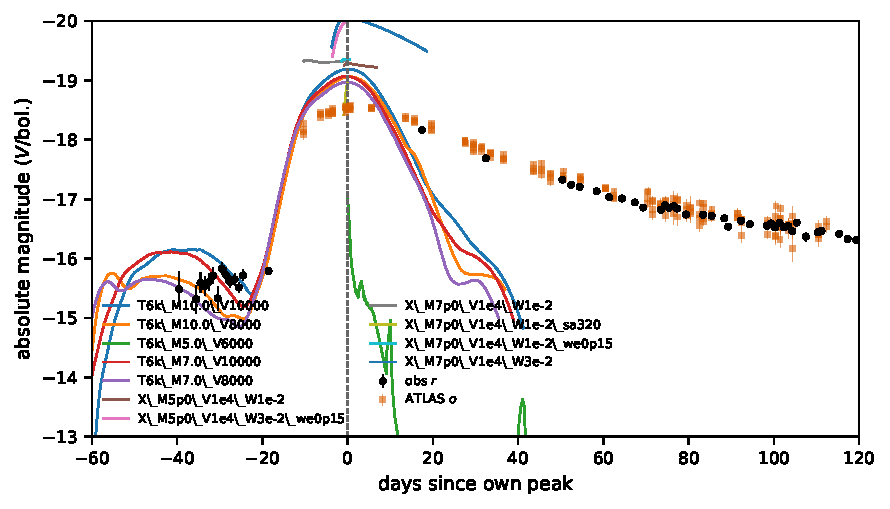
\includegraphics[width=\columnwidth]{figures/fig_grid.pdf}
  \caption{Grid lightcurves (model $V$ or bolometric magnitude, phased to each
  model's own peak) versus the observed $r$-band and ATLAS $o$ photometry.
  Shell kinetic energy sets the peak height, the wind column the post-peak
  decline, and \texttt{we\_transition\_dex} the sharpness of the rise.  Some
  \texttt{X\_*} runs are still in progress; truncated curves reflect completed
  STELLA time only.}
  \label{fig:grid}
\end{figure}

Figure~\ref{fig:grid} compares the current grid to the observations.  The
parameter roles established so far are: peak height $\leftarrow$ shell
kinetic energy; rise to main peak $\leftarrow$ \texttt{we\_transition\_dex}
(sharper interface $\rightarrow$ faster turn-on of dissipation); post-peak
decline $\leftarrow$ wind column (higher $\dot M$ $\rightarrow$ longer
diffusion and sustained $\rho v^3$ dissipation); first-bump duration
$\leftarrow$ wind gap size, fixed by the 400~d \SNa\ age and modified by
$\dot M$ and shell energetics.

\section{Open points and caveats}
\label{sec:open}

\begin{itemize}
  \item \textbf{Timeline convention.}  \texttt{source\_age\_days=400} places
    the shell launch $\sim$40~d after the observed \SNb\ peak if taken
    literally against the MJD~60490 explosion date; the physically meaningful
    constraint is the $\sim$330--360~d gap between the two events.  Model
    phases are always plotted relative to each model's own main peak.
  \item \textbf{Band mismatch.}  Model curves are Johnson--Cousins $R/V$ from
    STELLA; the observations are SDSS $r/g$ and ATLAS $o$.  Expect
    0.1--0.3~mag systematic offsets.
  \item \textbf{No \Ni\ tail.}  \SNb\ \Ni\ is set to $10^{-4}~\Msun$; if the
    observed tail is under-luminous after the wind/grid exploration, a real
    \Ni\ floor ($\sim0.02$--$0.05~\Msun$) is a separate lever.
  \item \textbf{Spectral attribution pending.}  The scenario's key test ---
    whether the radiatively heated \SNa\ ejecta produces the observed metal
    absorption at \SNa\ velocities --- awaits CMFGEN \citep{Hillier1998,
    Dessart2015} snapshots from the selected lightcurve model.  Line
    identification (ion, transition, formation depth, velocity) and a
    comparison of \SNa-only, \SNb-only and interaction spectra are required
    before the hypothesis can be accepted.
\end{itemize}

\bibliographystyle{aasjournal}
\bibliography{references}

\end{document}
